\section{Microstructure annotation}
\label{sec:microstructure_annotation_appendix}

% Microstructures represent logically structured argumentative claims
% \citep{boltuzic2017toward}.
% One can expresses logically equivalent claims in language. 
% To limit the language variation microstructures were designed to translate
% expression rich phrases to be translated to a restricted language to allow for
% easier inference. 
% - microstructures  consist of domain specific concepts, 
% connected through a finite set of argumentative relations, expressed using 
% a certain modality \\
% - microstructure annotation proceduced the microstructures data (
% see item element in \ref{item:microstructures_dataset})\\

\subsection*{Cheat sheet}

\begin{minted}{microstructure_lexer.py:MicroStructureLexer -x}
viewpoint_1(
	viewpoint_2[holder](
		relation_1([quantity_1] concept_1, [quantity_2] concept_2)
	)
)

concept_1 = concept OR relation_2(concept_3, concept_4)
concept_2 = concept OR relation_3(concept_5, concept_6)

\end{minted}

\noindent \textbf{Viewpoints} \\
- Believes, Approves, Disapproves, Desires

\begin{minted}{microstructure_lexer.py:MicroStructureLexer -x}
viewpoint_1(
	relation_1(relation_2(concept_3, concept_4), concept_2)
)
\end{minted}

\noindent \textbf{Relations} (grayed columns indicate dual meaning between relations in each row)

\begin{table}[!htb]
\begin{tabular}{|c c c c c c|}
\hline
\cellcolor{gray!25} \texttt{promotes} & \cellcolor{gray!25}\texttt{allow} & \texttt{purpose} & \texttt{equal} & \cellcolor{gray!25}\texttt{entails}     & \texttt{has\_associated} \\
\cellcolor{gray!25} \texttt{suppress} & \cellcolor{gray!25}\texttt{deny}  &         &       & \cellcolor{gray!25}\texttt{contradicts} &  \\
\hline
\end{tabular}
\end{table}

\noindent \textbf{Negation} (use with relations)
Use with relation in front (\texttt{not\_promotes}, \texttt{not\_suppress}, \dots) \\
 
\noindent \textbf{Quantities} (use with concepts) \\
- Some, All, Minority, Majority \\
          
\noindent \textbf{Concepts}\footnote{\url{https://docs.google.com/document/d/1ETobyCA4mpMmml1HXyxD7IG67EzrNK7W_2gzaIN0k_k/edit}} \\

\noindent \textbf{Quality} $\in [1, 5]$ \\
 
\noindent \textbf{Stance} $ \in {-2, -1, 0, 1, 2}$ \\

\pagebreak

\subsection*{Task description}

In this task we annotate argumentative sentences/claims and represent them
using a logical generative grammar language, as well as a stance. The
argumentative sentences are paraphrases of debate post excerpts. We will
provide you with the original post, as the argumentative sentences provided
might not be enough to fully understand the meaning. 
The language has a set of syntactic rules, which need to be respected. The
syntax of your solutions will be checked as you annotate the document. 
An example sentence will look like:
\noindent\begin{tabular}{@{}lp{0.8\columnwidth}}
(ex. 1) & \textit{Homosexual marriage can not truly be a marriage.}
\end{tabular} \vspace{0.4cm}

\noindent We want to translate this to the form of: 

\begin{tabular}{@{}m{1.5cm}  m{4.5cm}}
(ex. 1) &  \begin{minted}{microstructure_lexer.py:MicroStructureLexer -x}
believes(
    contradicts(homosexual marriage, marriage)
)
\end{minted}
\end{tabular}

In this context, we call homosexual marriage and marriage concepts. The element
contradicts is a relation between the concepts. Believes is a viewpoint that
depicts the author's perspective. See more on concepts, relations and
viewpoints in the language description section below. 

Good practice when creating these annotations is attempting to read them back
in natural language. In this case, we get: I believe that homosexual marriage
is not marriage.  If we compare this to the original sentence, we see that it
captures the essence of the example sentence (ex. 1). The wording is lost,
which can mean a lot sometimes (reading between the lines), but this is
something we’re OK with.

\subsection*{Language description}

As said, we annotate:
\begin{itemize}
\item Concepts
\item Relations between concepts
\item Viewpoints
\end{itemize}

\subsubsection*{Concepts}

Concepts are noun phrases mentioned when discussing a topic. We provide a set
of concepts that we have previously identified for the ``gay rights'' topic\footnote{
Concepts available at 
\url{https://docs.google.com/document/d/1ETobyCA4mpMmml1HXyxD7IG67EzrNK7W_2gzaIN0k_k/edit?usp=sharing}
}
Some concepts are tab-shifted, which you can disregard, some have
slashes between them (i.e. \texttt{heterosexual marriage} / \texttt{traditional marriage}); we
consider these synonyms, please choose the first one. Your task is to search
through this list and find appropriate concepts (as close concept as possible)
mentioned in the input sentence and associate the appropriate relations between
them. Some example concepts: \texttt{procreation}, \texttt{reproduction}, \texttt{adoption}, \texttt{homosexual}
\texttt{adoption}, \texttt{have children}, \texttt{gay people}. 
If you feel you need to use a concept not
in the list, please contact us with the example. Another case would be where a
concept might be implicit, in the sentence: \textit{Allow gay marriages}, we recognize
the relation \texttt{allow} (explained in relations below) and the concept \texttt{gay marriages}
(argument B for relation \texttt{allow}).  We don’t know what the principle is, but from
the topic we know the state can allow gay marriages, therefore we can translate
the sentence as: \texttt{allow(state, gay marriage).}

\subsubsection*{Quantity}

Each concept can be expressed with quantity. Quantities allowed are:
\begin{itemize}
\item Some 
\item All
\item Minority
\item Majority
\end{itemize}

\begin{table}[!htb]
\begin{tabular}{@{}m{1.5cm} m{5cm} m{8cm}}
\toprule
Example & Sentence & Microstructure \\
\midrule
(ex. 2.a) & Some people promote gay marriages. & 
\begin{minted}{microstructure_lexer.py:MicroStructureLexer -x}
believes(
  promote([some]people, gay marriage)
) 
\end{minted}
\\
(ex. 2.b) &Democracy helps the majority of people. &
\begin{minted}{microstructure_lexer.py:MicroStructureLexer -x}
believes( 
  promote(democracy, [majority] people)
)
\end{minted} 
\\
\bottomrule
\end{tabular}
\end{table}

\subsubsection*{Relations}

Relations are connections between concepts. Relations are not domain-bound (one
can use them outside of gay marriages), while concepts are tied to domain 
(\texttt{gay marriages} in this case). Relations are verb phrases. 
Possible relations are:

\begin{footnotesize}
\begin{tabular}{lp{5cm}p{2.5cm}p{3cm}}
\toprule
Relation & Explanation & Argument A & Argument B \\
\midrule
\texttt{promotes(A, B)} & 
\makecell[cl]{
\textbf{A} promotes / fosters / \\
brings about / leads \\ 
/ forces / advances \\
/ increases /encourages \\
/ boosts / increases \\
the likelihood of / causes \textbf{B}  \\ \\
``Soft causation'' \\\\
\href{https://framenet2.icsi.berkeley.edu/fnReports/data/frameIndex.xml?frame=Cause_change_of_position_on_a_scale}{FrameNet link} 
}
& 
Agent (which promotes) & 
Attribute (what gets promoted) \\
\midrule
\texttt{suppress(A, B)} & 
\makecell[cl]{
\textbf{A} suppresses / decreases \\ 
likelihood / smothers / \\
represses / puts down / \\
vanquishes \textbf{B} 
}
&
Agent (which suppresses) & 
Attribute (what gets suppressed)
\\
\midrule
\texttt{allow(A, B)} & 
\makecell[cl]{
Principle \textbf{A} \\ 
allows / approves / \\
licenses \textbf{B} \\\\
\href{https://framenet2.icsi.berkeley.edu/fnReports/data/frameIndex.xml?frame=Prohibiting_or_licensing}{FrameNet link}
} & 
Principle
& 
State of affairs \\
\midrule
\texttt{deny(A, B)} & 
\makecell[cl]{
Principle \textbf{A} \\
denies / disallows /
bans \textbf{B} } & 
Principle & 
State of affairs\\
\midrule
\texttt{entails(A, B)} & 
\makecell[cl]{
State of affairs \textbf{A} \\
necessarily, per definition \\
or causally, makes \textbf{B} true \\\\
Proposition \textbf{B} has \\
support \textbf{A} \\\\
\href{https://framenet2.icsi.berkeley.edu/fnReports/data/frameIndex.xml?frame=Evidence}
{FrameNet link}
}
& State of affairs & Implication \\
\midrule
\texttt{contradicts(A, B)} & 
\makecell[cl]{
State of affairs \textbf{A} \\
makes \textbf{B} not true}
& State of affairs & Contradiction \\
\midrule
\texttt{purpose(A, B)} & 
\makecell[cl]{The purpose of \textbf{A} is \textbf{B} \\\\
\href{https://framenet2.icsi.berkeley.edu/fnReports/data/frameIndex.xml?frame=Purpose
}{FrameNet link}
} & Agent & Goal \\
\midrule
\texttt{has\_associated(A, B)} &
\makecell[cl]{
\textbf{A} has properties affected by \\
the existence of \textbf{B} \\\\
\href{https://framenet2.icsi.berkeley.edu/fnReports/data/frameIndex.xml?frame=Membership
}
{Similar FrameNet definition} 
} & Group & Member \\
\midrule
\texttt{equal(A, B)} & \textbf{A} is equal to \textbf{B} & Concept \textbf{A} & Concept \textbf{B} \\
\bottomrule
\end{tabular}
% \caption{Relation definition table}
% \label{tab:relation_definition}
% \end{table}
\end{footnotesize}

\subsubsection*{Negation}
%TODO proper references in table rows

Relations can be negated to indicate opposite meaning. Notice how example $3.a$
is not saying it is suppressing, but just denied promoting. Example $3.b$ also can’t
use contradicts since being happy does not imply you are not rich, but it does
not imply you are.

\begin{table}[h!]
\begin{footnotesize}
\begin{tabular}{@{}m{1.5cm} m{5cm} m{8cm}}
\toprule
Example & Sentence & Microstructure \\
\midrule
(ex. $3.a$) & \textit{Marijuana does not help cure cancer. } & 
\begin{minted}{microstructure_lexer.py:MicroStructureLexer -x}
believes(
  not_promotes(marijuana, cure cancer)
)
\end{minted}
\\
(ex. 3.b) & \textit{If you are happy, doesn’t mean you’re rich.} 
 &
\begin{minted}{microstructure_lexer.py:MicroStructureLexer -x}
believes(
  not_entails(feel happy, be rich)
)
\end{minted} 
\\
\bottomrule
\end{tabular}
\end{footnotesize}
\end{table}

\subsubsection*{Nested Relations}

Relations can be nested within each other. Each relation takes two arguments.
An argument can be another relation or a concept. Make sure you are correct
with closing the opened braces. 

\begin{table}[h!]
\begin{footnotesize}
\begin{tabular}{@{}m{1.5cm} m{5cm} m{8cm}}
\toprule
Example & Sentence & Microstructure \\
\midrule
(ex. $4.a$) & \textit{I think allowing gay marriages promotes freedom. } & 
\begin{minted}{microstructure_lexer.py:MicroStructureLexer -x}
believes(promotes(
  allow(state, gay marriage), freedom
  )
)
\end{minted}
\\
(ex. 4.b) & \textit{The purpose of life is to allow having freedom.} 
 &
\begin{minted}{microstructure_lexer.py:MicroStructureLexer -x}
believes(
  purpose(life, 
    allow(state, freedom)
  )
)
\end{minted} 
\\
(ex. 4.c) & \textit{It’s the same thing to allow gay marriages or heterosexual marriages.} & 
\begin{minted}{microstructure_lexer.py:MicroStructureLexer -x}
believes(
  equal(
    allow(state, gay marriage), 
    allow(state, heterosexual marriage)
  )
)
\end{minted}
\\
\bottomrule
\end{tabular}
\end{footnotesize}
\end{table}

\subsubsection*{Viewpoints}

Viewpoints reflect whether the a viewpoint holder thinks the claim is believed
(fact), desired (policy), or considered right/wrong (value judgement). When not
mentioned, the claim holder is considered to be the author of the argumentative
sentence. If not, one needs to annotate the claim holder next to the viewpoint
type (\textit{I believe the Bible states}, \textit{I think the state of Florida should}), which
we call second-level viewpoints. Second-level viewpoints are annotated together
with a concept, for example: "\textit{I saw that the Bible states: It should be
allowed}" corresponds to "\texttt{believes(believes[Bible]...))}".
Possible viewpoints are \\

\begin{tabular}{l p{7cm} p{6cm}}
\toprule
Viewpoint & Description & Example \\
\midrule
\textbf{believes} & \textbf{A} believes / argues / thinks
that claim \textbf{C} is true & 
I believe people are mortal. \\
\midrule
\textbf{desires} & 
\textbf{A} believes / argues / thinks \textbf{C} 
should be true in the future or should remain true
& People should be nicer \\
\midrule
\textbf{approves} & 
\textbf{A} believes / argues / thinks \textbf{C} 
is morally / ethically right & Forgiving is bad \\
\midrule
\textbf{disapproves} & 
\textbf{A} believes / argues / thinks \textbf{C} 
is morally / ethically wrong & 
Drugs are bad.  \\
\bottomrule
\end{tabular} \\
% \label{tab:viewpoints}
% \caption{Viewpoints, their descriptions and examples of using specific viewpoints in claims}

\noindent Annotating a claim holder explicitly should be done like for sentence:

\begin{table}[h]
\begin{tabular}{@{}m{1.5cm} m{5cm} m{8cm}}
\toprule
Example & Sentence & Microstructure \\
\midrule
(ex. $5.a$) & \textit{I saw the Bible claims gay people are equal to straight people} & 
\begin{minted}{microstructure_lexer.py:MicroStructureLexer -x}
believes(
  believes[Bible](
    equal(gay people, straight people)
  )
)
\end{minted}
\\
\bottomrule
\end{tabular}
\label{tab:viewpoint_example}
\caption{Viewpoint claim annotation example}
\end{table}

\subsubsection*{Stance}

Please annotate stance, which answers the question:
\textbf{Is the sentence pro-gay or not just by looking only at the offered claim} (not
the entire post context)? Stance $\in {-2, -1, 0, 1, 2}$.

\begin{table}[!htb]
	\centering
\begin{tabular}{c p{10cm}}
\toprule
Stance Value & Explanation \\
\midrule
-2 & The author or the viewpoint of the second person is definitely against the
claim (explicitly states so). Any form of discrimination is seen as against.  \\
-1 & There is some implication that the author might be against gay rights  \\
0 & There is no stance towards gays, stance is bipolar \\
1 & Reverse of -1 \\
2 & Reverse of -2 \\
\bottomrule
\end{tabular}
\label{tab:stance}
\caption{Possible stance values with explanations}
\end{table}

\begin{table}[!htb]
	\centering
\begin{tabular}{c p{10cm} r}
\toprule
Example & Claim & Stance \\
\midrule
(ex. $6.a$) &  I think allowing gay marriages promotes freedom. & 2 \\
(ex. $6.b$) & All people are equal. & 0 \\
(ex. $6.c$) & Allowing gay marriages will be the end of us all. &  -2 \\
(ex. $6.d$) & I would ban religious gay marriage. & -2 \\
(ex. $6.e$) & The Bible is against gay marriages & -2 \\
\bottomrule
\end{tabular}
\label{tab:stance_example}
\caption{Examples of stance for the gay marriages topic}
\end{table}

\subsubsection*{Quality}

Evaluate your own logical claim transformation by inputting a number $\in [1, 5]$
rating how well does the proposed formalization suit what the person said?

\subsection*{Technical instructions}

You will be provided with an excel spreadsheet with the posts and sentences.
Please notify us as soon as possible if you can’t use Excel --- we can send you
the annotation in another format (Google spreadsheet, etc.). 

The goal is to fill up the E, F, G columns (logical representation, stance and
quality, highlighted in green) in the provided spreadsheet based on the
argumentative sentence in column D. Feel free to ignore columns A, and C (used
for internal tracking). Column B might be useful, if you can’t determine the
meaning in D. If you have problems or comments about an example, feel free to
add them in column H and raise questions with us --- we will be happy to
discuss! An example row will look like in table~\ref{tab:annotation_example}

\begin{table}[!htb]
\scriptsize
\begin{tabular}{|p{1.5cm} | p{2cm} | p{2cm} | p{2cm} | p{2cm} |c| c| c|}
\toprule
A & B & C & D & E & F & G & H \\
\midrule
POST ID & POST TEXT & SEGMENT ID & SENTENCE & LOGICAL REPRESENTATION
& STANCE & QUALITY & COMMENTS \\
\midrule
A75.data & 
Here we is the full text of the post. This will be relatively long.
This is divided into segments (argumentative sentences) that you then annotate. 
& 758 & 
The full text of the post will be relatively long.  
& \cellcolor{green!25} &  \cellcolor{green!25}& \cellcolor{green!25} & \cellcolor{green!25} \\
\bottomrule
\end{tabular}
\caption{Example excel sheet to annotate}
\label{tab:annotation_example}
\end{table}

A syntax checking script and your annotation is packaged into a zip file.  Your goal is to
fill column E in \texttt{annotation.xls}.

\subsubsection*{Checking syntax correctness (optional)}

We provide a script to verify that your solutions are syntactically correct. 
You will need to install python and a python library xlrd. Make sure to install
\texttt{python 2.x}!

If you are not familiar with python, installing them on Windows is described in
\url{http://www.howtogeek.com/197947/how-to-install-python-on-windows/}
Xlrd is available to install from:
\url{http://www.lexicon.net/sjmachin/xlrd-0.6.1.win32.exe} 
To install it, you will need to Run-as-administrator. 
Please contact us if you have issues installing these. 
To help check correctness of your solution, we offer a python script that can
be run in two ways:

\begin{description}[style=multiline, labelwidth=1.5cm]
\item[\namedlabel{item:excel}{All}] Check all solutions in your excel spreadsheet
\item[\namedlabel{item:single_claim}{Single}] Check a single claim
\end{description}

\begin{figure}
	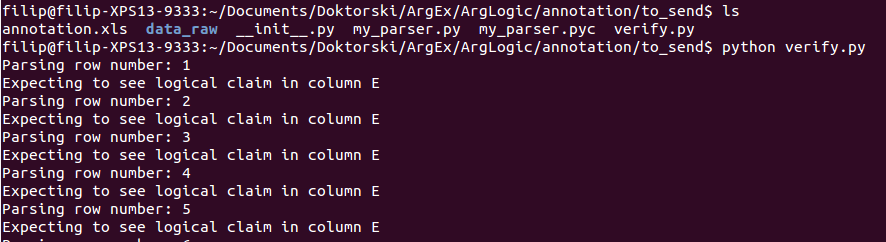
\includegraphics[scale=0.5]{struc_instructions_1.png}
	\caption{Expected output of running microstructure syntax check on entire file (\ref{item:excel}) mode}
	\label{fig:struc_instructions_all}
\end{figure}

\begin{figure}
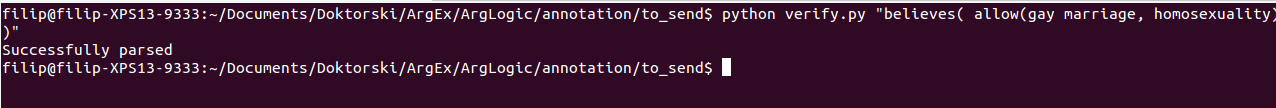
\includegraphics[scale=0.35]{struc_instructions_2.png}
	\caption{Expected output of running microstructure syntax check on a
	\label{fig:struc_instructions_2}
	single claim (\ref{item:single_claim} mode) }
\end{figure}

\noindent The script and your annotation is packaged into a zip available here. When you
unzip it, you should input your solutions in excel file \texttt{to\_send/annotation.xls}
To run it in \ref{item:excel} mode simply run \texttt{python verify.py} while
positioned in the \texttt{to\_send} directory using the command line (shown in
figure~\ref{fig:struc_instructions_all}) To run in \ref{item:single_claim}
mode, also position yourself in the \texttt{to\_send/} directory, but run as
shown in figure~\ref{fig:struc_instructions_2}.
